\documentclass{article}
\usepackage{graphicx}
\begin{document}

\title{
Bryan Petzinger \\
Computer Vision \\
HW3 \\
}
\maketitle

\section{Writeup}
This program reads in a raw image, performs eroison and dilation operations to obtain the morphological skeleton, and then reconstructs the original image from that skeleton using further erosion and dilation operations. \\

Program is written in java and has methods for the following operation: Erosion, dilation, open, close, set union, set difference, test if a set is empty as well as methods for reading/writing a raw image to/from file. Based on those methods, the algorithms discussed in class were implemented for discovering the morphological skeleton of an image and restoring an image from its morphological image. \\

The creation of a skeleton is done recursively, and each Sn is pushed onto a stack. Each Sn from the stack is then unioned together to obtain the skeleton. Later the stack is used again to reconstruct the image. There is a memory optimization that is possible where each Sn is stored in a single array, instead of a stack of arrays, by writing the N value into the array. However I ran into an issue with this implementation and ran out of time so I just used a stack as it was quicker to implement. \\

The final program works correctly, I did a binary diff on the original image and reconstructed image and they were identical. \\

I ran into some bugs dealing with the raw image format, intially reading the value in backwards (so I was effectively finding the skeleton of the backgroun). Later I had an issue that worked out to writing an incorrect byte value for the background which was caused by the OutputStream I was using writing a signed byte (values -126 to 127 instead of 0 to 255). Both of these issues took me awhile to discover the root cause, and besides them the implementation of the actual logic was fairly straightforward. \\

\section{Figures}

\begin{figure}[h]
\caption{}
\centering
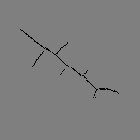
\includegraphics{images/skeleton.jpg}
\end{figure}

\begin{figure}[h]
\caption{}
\centering
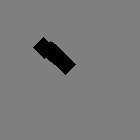
\includegraphics{images/rebuilt_image10.jpg}
\end{figure}

\begin{figure}[h]
\caption{}
\centering
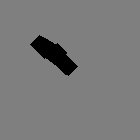
\includegraphics{images/rebuilt_image9.jpg}
\end{figure}

\begin{figure}[h]
\caption{}
\centering
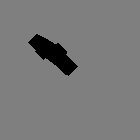
\includegraphics{images/rebuilt_image8.jpg}
\end{figure}

\begin{figure}[h]
\caption{}
\centering
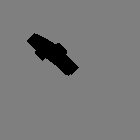
\includegraphics{images/rebuilt_image7.jpg}
\end{figure}

\begin{figure}[h]
\caption{}
\centering
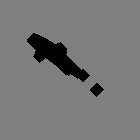
\includegraphics{images/rebuilt_image6.jpg}
\end{figure}

\begin{figure}[h]
\caption{}
\centering
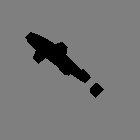
\includegraphics{images/rebuilt_image5.jpg}
\end{figure}

\begin{figure}[h]
\caption{}
\centering
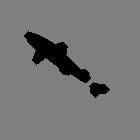
\includegraphics{images/rebuilt_image4.jpg}
\end{figure}

\begin{figure}[h]
\caption{}
\centering
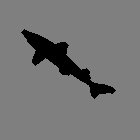
\includegraphics{images/rebuilt_image3.jpg}
\end{figure}

\begin{figure}[h]
\caption{}
\centering
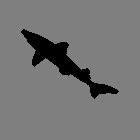
\includegraphics{images/rebuilt_image2.jpg}
\end{figure}

\begin{figure}[h]
\caption{}
\centering
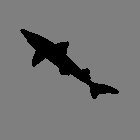
\includegraphics{images/rebuilt_image1.jpg}
\end{figure}

\begin{figure}[h]
\caption{}
\centering
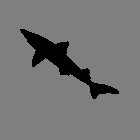
\includegraphics{images/rebuilt_image0.jpg}
\end{figure}








\end{document}
